
\section{Motivation}
\label{sec:motivation}



\subsection{An example of a commit }
\label{sec:examle}

\subsection{Convolutional Neural Networks}
\label{sec:background_cnn}

\begin{figure*}[t!]
	\center
	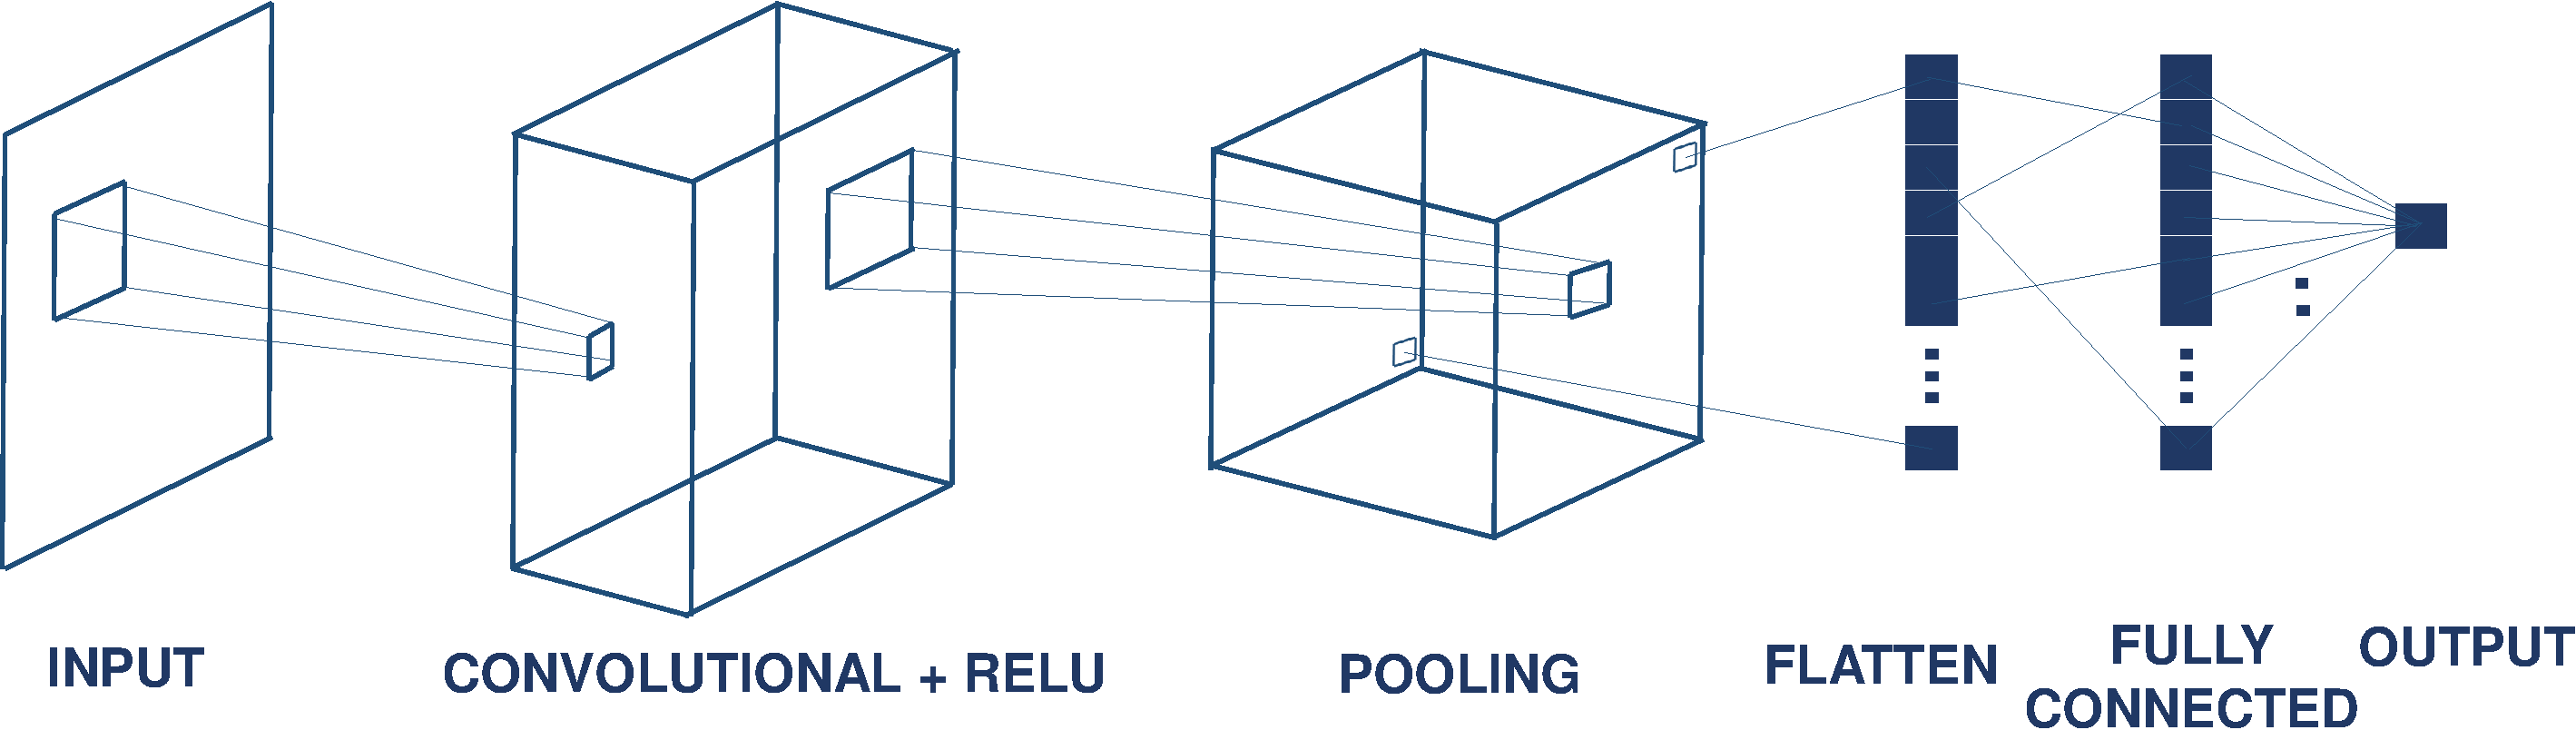
\includegraphics[scale=0.3]{figs/cnn.pdf}
	\caption{A simple convolutional neural network architecture.}
	\label{fig:cnn}
\end{figure*}

\begin{figure}[t!]
	\center
	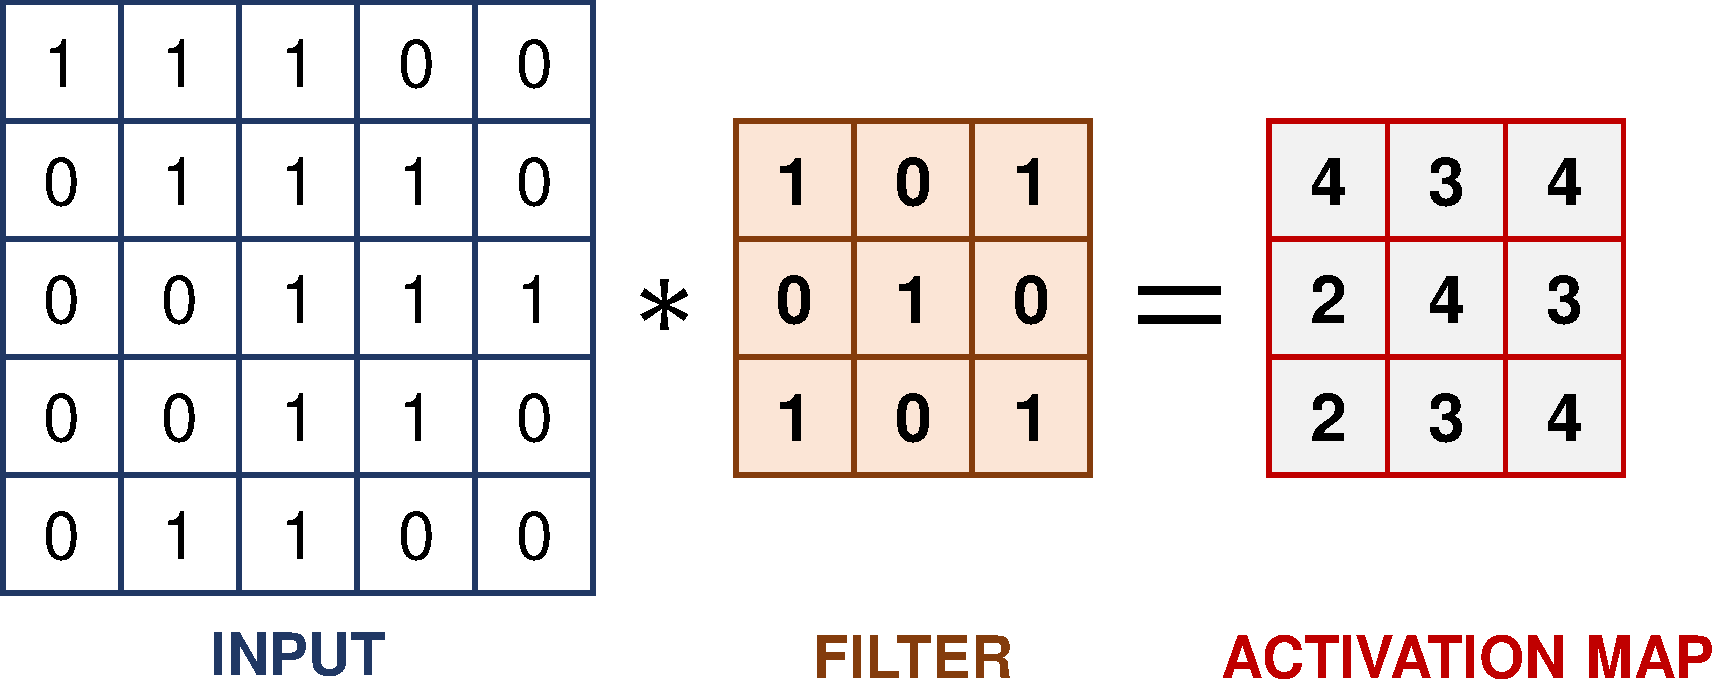
\includegraphics[scale=0.27]{figs/filter.pdf}
	\caption{An example of a convolutional layer in CNN.}
	\label{fig:filter}
\end{figure}

One of the most powerful forms of deep learning neural networks is the Convolutional Neural Network (CNN)~\cite{lecun2015deep}. CNNs are widely used to solve image pattern recognition problems and have been achieved significant results~\cite{karpathy2014large, lawrence1997face, krizhevsky2012imagenet}. Like traditional deep learning networks, CNNs receive an input and perform a product operation followed by a nonlinear function. The last layer is the output layer containing objective functions~\cite{zhao2017loss} associated with the labels of the input.

Figure~\ref{fig:cnn} illustrates a simple CNN for classification task. The simple CNN includes an input layer, a convolutional layer, followed by the rectified linear unit (RELU) which is a nonlinear activation function, a pooling layer, a fully-connected layer, and an output layer in the following paragraphs. 

The input layer takes an input as 2-dimensional array or 3-dimensional array and passes it through a of convolution layers.

The convolutional layer plays a vital role in CNN and it takes advantage of the use of learnable filters. These filters are small in spatial dimensionality, but they are applied along the entirety of the depth of the input data. For example, given an input data $\textbf{I} \in \mathbb{R}^{\text{H} \times \text{W} \times \text{D}}$ and a filter $\textbf{K} \in \mathbb{R}^{\text{h} \times \text{w} \times \text{D}}$, we produce a new activation map $\textbf{A} \in \mathbb{R}^{(\text{H} - \text{h}) \times (\text{W} - \text{w}) \times 1}$. Figure~\ref{fig:filter} presents a visual representation of a convolutional layer in CNN. The RELU is then applied to each value of the activation map as follows:
\begin{equation}
\label{eq:relu}
f(x) = max(0, x)   
\end{equation}

The pooling layer aims to reduce 

reduce the dimensionality of the representation, and thus further reduce the number of parameters and the computational
complexity of the model.







